\documentclass[reqno]{amsart}
\usepackage{amsmath,amssymb,amsfonts,amsthm}
\usepackage{eucal}
\usepackage{graphicx,psfrag}
\usepackage{hyperref}
\usepackage{multirow}
\usepackage{verbatim} 
\usepackage{empheq}
\usepackage{lipsum}
\usepackage{color}

\theoremstyle{definition}
\newtheorem{lem}{Lemma}[section]
\newtheorem{cor}[lem]{Corollary}
\newtheorem{prop}[lem]{Proposition}
\newtheorem{thm}[lem]{Theorem}
\newtheorem{eg}{Example}
%\newtheorem{eg}[lem]{Example}

\definecolor{myblue}{rgb}{.8, .8, 1}
\newcommand*\mybluebox[1]{\colorbox{myblue}{\hspace{1em}#1\hspace{1em}}}
\newcommand*\widefbox[1]{\fbox{\hspace{1em}#1\hspace{1em}}}

\numberwithin{equation}{section}

\newcommand\tr{\mathrm{tr}}
\newcommand\bip{\mathrm{bip}}
\newcommand\rank{\operatorname{rank}}

\begin{document}

\title{``LIATE" and Tabular Intergration By Parts}

%\author{Nathan Reff}
\address{Nathan Reff\\Department of Mathematics\\Alfred University\\ Alfred, NY 14802, U.S.A.}
\email{reff@alfred.edu}

%\date{\today}
\maketitle

\section{LIATE}
The {\bf LIATE} method was first mentioned by Herbert E. Kasube in \cite{Kasube}.  The function that appears first in the following list should be $u$ when using integration by parts:

\begin{center}
\begin{tabular}{ |c|l|l|}
\hline
  {\bf L} & Logatithmic functions  &  $\ln(x)$, $\log_2(x)$, etc. \\
\hline
  {\bf I} & Inverse trig. functions  &  $\tan^{-1}(x)$, $\sin^{-1}(x)$, etc. \\
\hline
  {\bf A} & Algebraic functions  &  $x$, $3x^2$, $5x^{25}$, etc. \\
\hline
  {\bf T} & Trig. functions  &  $\cos(x)$, $\tan(x)$, etc. \\
\hline
  {\bf E} & Exponential functions  &  $e^x$, $2^x$, etc. \\
\hline
\end{tabular}
\end{center}

\begin{eg}  \[ \int x\sin(x) dx.\]

Following the LIATE method, $u=x$ and $dv=\sin(x)dx$ since $x$ is an {\bf a}lgebraic function and $\sin(x)$ is a {\bf t}rigonometric function.  Therefore,

\begin{center}
  \begin{tabular}{ r||l}
    $u=x$ & $dv=\sin(x) dx$ \\ 
    $du=dx$ & $v=-\cos(x)$\\ 
  \end{tabular}
\end{center}
\noindent and 
\begin{align*} \int x \sin(x) dx &= -x \cos(x) - \int (-\cos(x)) dx \\
&= -x \cos(x) + \sin(x) +C.
\end{align*}
\end{eg}

\vspace{1pc}
\hrule
\vspace{1pc}

\begin{empheq}[box=\widefbox]{align}
\text{{\bf WARNING:}  This technique is not perfect!}
\end{empheq}
There are exceptions to LIATE.  Some of these can be solved using the order ``ILATE" instead.  Sometimes, something completely different needs to be considered.

\begin{eg} \[ \int x^3 e^{x^2} dx.\]

Following the LIATE rule, $u=x^3$ and $dv=e^{x^2}dx$.  However, we would actually set $u=x^2$ and $dv=xe^{x^2}$.

\begin{center}
  \begin{tabular}{ r||l}
    $u=x^2$ & $dv=xe^{x^2} dx$ \\ 
    $du=2xdx$ & $v=\frac{1}{2}e^{x^2}$\\ 
  \end{tabular}
\end{center}

and so 
\begin{align*} \int x^3 e^{x^2} dx &= x^2 \left(\frac{1}{2}e^{x^2}\right) - \int \frac{1}{2}e^{x^2} 2xdx \\
&= \frac{1}{2} x^2 e^{x^2} - \int xe^{x^2} dx \\
&= \frac{1}{2} x^2 e^{x^2} - \frac{1}{2}e^{x^2} + C\\
&= \frac{1}{2}e^{x^2}(x^2-1) +C.
\end{align*}
\end{eg}

\vspace{1pc}
\hrule
\vspace{1pc}
\begin{eg} \[ \int \sec^3(x) dx.\]

Following the LIATE rule, $u=1$ and $dv=\sec^3(x)dx$.  However, we would actually set $u=\sec(x)$ and $dv=\sec^2(x)$.

\begin{center}
  \begin{tabular}{ r||l}
    $u=\sec(x)$ & $dv=\sec^2(x) dx$ \\ 
    $du=\sec(x)\tan(x)dx$ & $v=\tan(x)$\\ 
  \end{tabular}
\end{center}

and so 
\begin{align*} \int \sec^3(x)dx &= \sec(x)\tan(x) - \int \tan^2(x)\sec(x)dx \\
&= \sec(x)\tan(x) - \int (\sec^2(x)-1)\sec(x)dx \\
&= \sec(x)\tan(x) - \int \big(\sec^3(x)-\sec(x)\big)dx \\
&= \sec(x)\tan(x) - \int \sec^3(x)dx+\int\sec(x)dx \\
&= \sec(x)\tan(x) - \int \sec^3(x)dx+\ln|\sec(x)+\tan(x)|. \\
\end{align*}
Since the integral we are solving reappears, we need to add it to the left side to get
\[ 2\int \sec^3(x)dx =\sec(x)\tan(x) +\ln|\sec(x)+\tan(x)|.  \]
Finally,

\[ \int \sec^3(x)dx =\frac{1}{2}\sec(x)\tan(x) +\frac{1}{2}\ln|\sec(x)+\tan(x)|  +C.\]

\end{eg}




\vspace{1pc}
\hrule
\vspace{1pc}

\section{Tabular Integration By Parts}

When integration by parts is needed more than once you are actually doing integration by parts recursively.  This leads to an alternative method which just makes the amount of writing significantly less.  I will explain this through the following example.

\begin{eg} Consider the integral
\[ \int x^3 \sin(x) dx.\]

Let $u=x^3$.  We make two columns, putting $u$ in the left column.  In the left column list all subsequent derivatives until zero is reached.  In the right column begin with $dv=\sin(x)$ and list each subsequent integral down to the same level as zero is in the left.

\begin{center}
\begin{tabular}{ |c|c|}
\hline
  Derivatives of $u$ & integrals of $dv$   \\
\hline
  $x^3$ & $\sin(x)$   \\
\hline
  $3x^2$ & $-\cos(x)$   \\
\hline
  $6x$ & $-\sin(x)$   \\
\hline
  $6 $& $\cos(x)$   \\
\hline
$0 $& $\sin(x)$   \\
\hline
\end{tabular}
\end{center}

Now pair the $1^{\text{st}}$ entry of the left column with the $2^{\text{nd}}$ entry of right column, the $2^{\text{nd}}$ entry of the left column with the $3^{\text{rd}}$ entry of the right column, etc.  Do this until no more pairs can be made.  It might be helpful to draw in arrows to see the pairing as follows:

\begin{center}
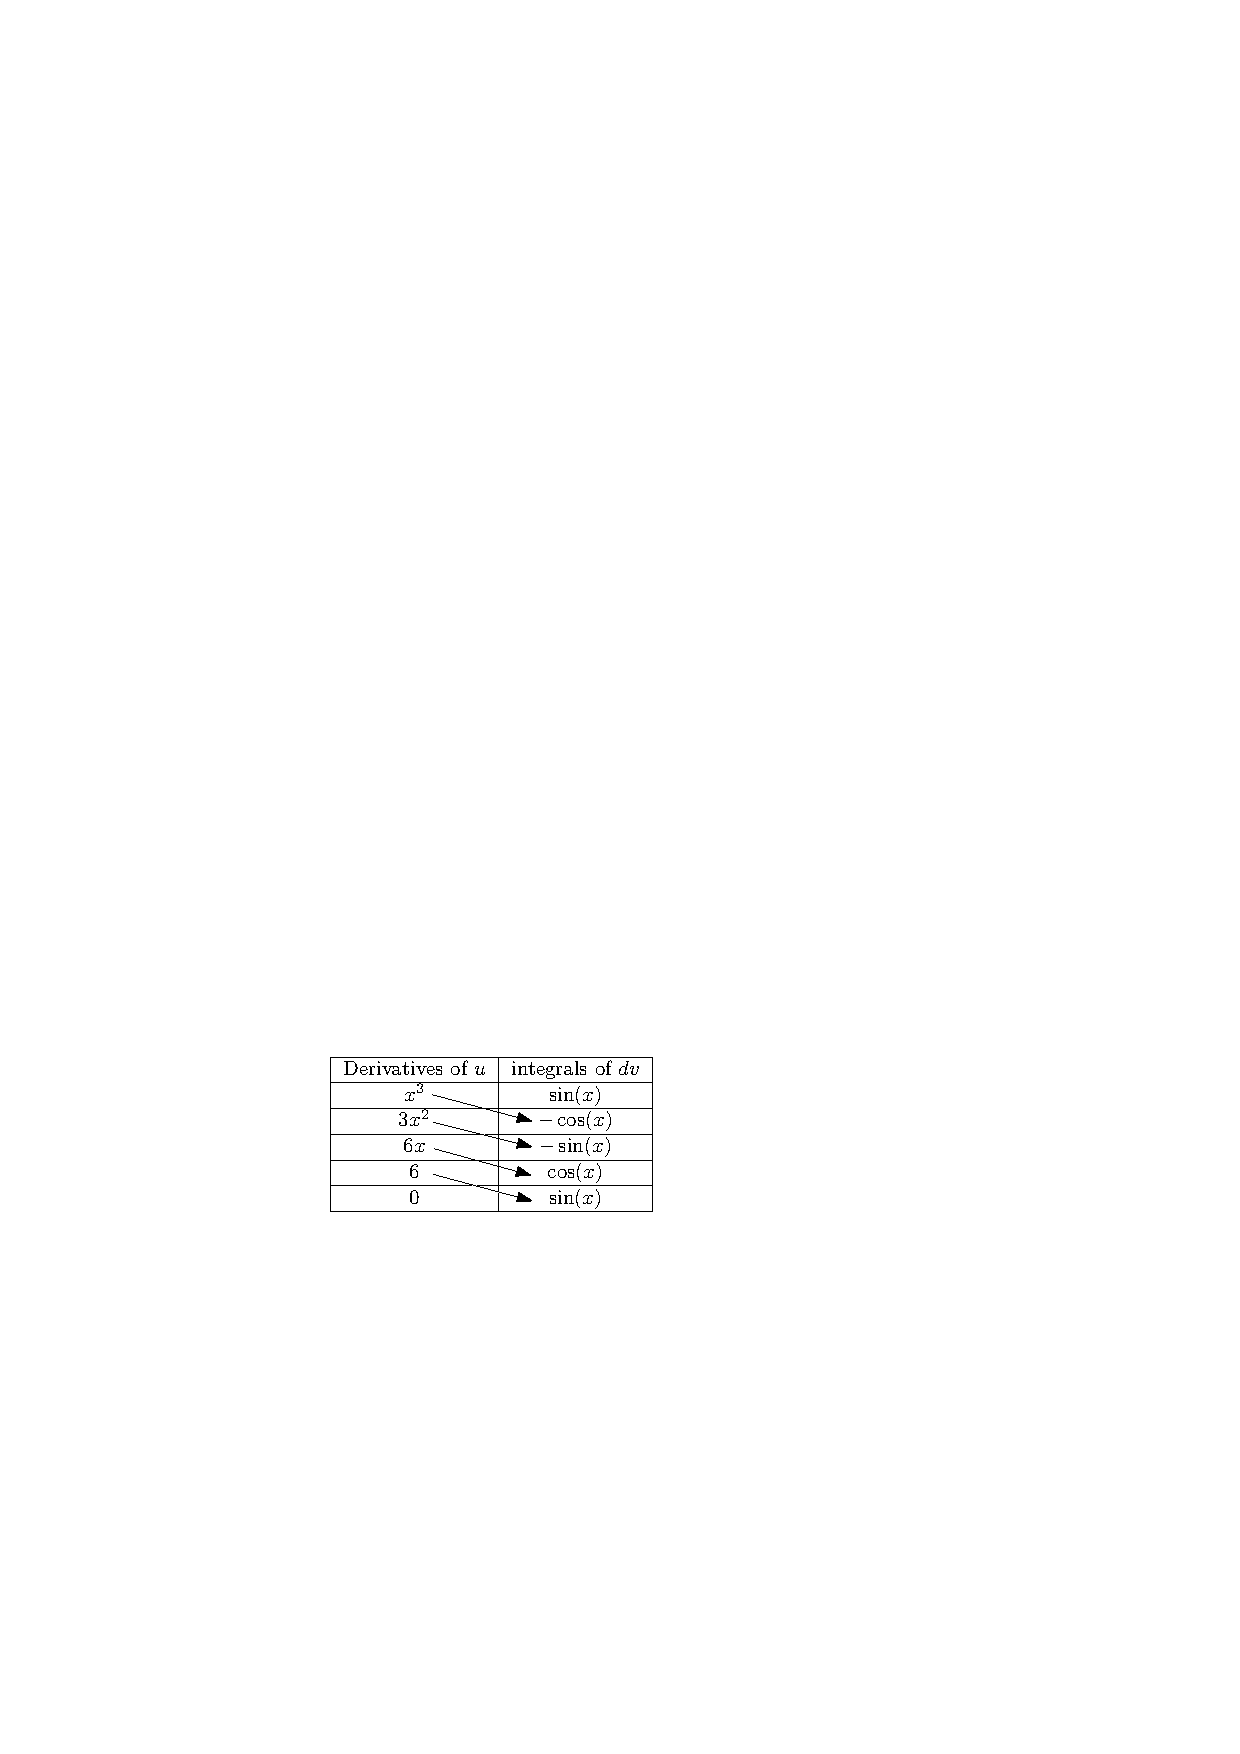
\includegraphics[scale=1]{TabEg}
\end{center}
Now add these pairs with \underline{{\bf alternating signs}} (beginning with the positive sign).  The result is the following (notice alternating signs):
\[ (+)(x^3)(-\cos(x))+(-)(3x^2)(-\sin(x))+(+)(6x)(\cos(x))+(-)(6)(\sin(x))+C \]

With simplification we have

\[ \int x^3 \sin(x) dx = -x^3\cos(x)+3x^2\sin(x)+6x\cos(x)-6\sin(x)+C. \]
\end{eg}

With a bit of work this can be extended to almost all recursive uses of integration by parts.  Even cases such as $\int \cos(x) e^x dx$ where a derivative of zero does not occur.  You can find many more examples on the web. 

\begin{thebibliography}{19}
\bibitem{Kasube} Herbert E. Kasube, A Technique for Integration by Parts, \emph{The American Mathematical Monthly},  {\bf 90} (1983). 210--211.
 

\end{thebibliography}

\end{document}
